%%%%%%%%%%%%%%%%%%%%%%%%%%%%%%%%%%%%%%%%%%%%%%%%%%%%%%%%%%%%%%%
%
% Welcome to Overleaf --- just edit your LaTeX on the left,
% and we'll compile it for you on the right. If you open the
% 'Share' menu, you can invite other users to edit at the same
% time. See www.overleaf.com/learn for more info. Enjoy!
%
%%%%%%%%%%%%%%%%%%%%%%%%%%%%%%%%%%%%%%%%%%%%%%%%%%%%%%%%%%%%%%%
% Author: Izaak Neutelings (May 2020)
% Inspiration: https://tex.stackexchange.com/questions/285578/how-to-draw-parallelepiped-and-cube-with-latex/288101#288101
\documentclass[border=3pt,tikz]{standalone}
\usetikzlibrary{arrows,arrows.meta}
\usetikzlibrary{calc}
\usetikzlibrary{decorations.markings}
\usetikzlibrary{angles,quotes} % for pic (angle labels)
%\usepackage{tkz-euclide} % for \tkzMarkRightAngle
%\usetkzobj{all}
\tikzset{>=latex} % for LaTeX arrow head

\colorlet{myblue}{blue!80!black}
\colorlet{mydarkblue}{blue!35!black}
\colorlet{myred}{black!50!red}
\colorlet{glasscol}{blue!10}
\colorlet{Ecol}{orange!90!black}
\tikzstyle{myarr}=[-{Latex[length=3,width=2]}]
\tikzstyle{Evec}=[Ecol,{Latex[length=2.8,width=2.5]}-{Latex[length=2.8,width=2.5]},line width=0.6]
\tikzstyle{glass}=[top color=glasscol!88!black,bottom color=glasscol,shading angle=0]
%\tikzstyle{glass}=[top color=glasscol!88!black,bottom color=glasscol,middle color=glasscol!98!black,shading angle=0]
\tikzset{
  light beam/.style={thick,myblue,decoration={markings,
                     mark=at position #1 with {\arrow{latex}}},
                     postaction={decorate}},
  light beam/.default=0.5}

\newcommand\rightAngle[4]{
  \pgfmathanglebetweenpoints{\pgfpointanchor{#2}{center}}{\pgfpointanchor{#3}{center}}
  \coordinate (tmpRA) at ($(#2)+(\pgfmathresult+45:#4)$);
  \draw[white,line width=0.6] ($(#2)!(tmpRA)!(#1)$) -- (tmpRA) -- ($(#2)!(tmpRA)!(#3)$);
  \draw[blue!40!black] ($(#2)!(tmpRA)!(#1)$) -- (tmpRA) -- ($(#2)!(tmpRA)!(#3)$);
}

% WAVEFRONT
\def\p{0.03}
\def\r{0.25}
\tikzset{
  wavefront/.pic={
    \tikzset{/wavefront/.cd,#1}
    \fill (0,0) circle (\p);
    \draw (\wang:\r) arc(\wang:-\wang:\r);
  }
  /wavefront/.search also={/tikz},
  /wavefront/.cd,
  ang/.store in=\wang, ang={60},
}


\begin{document}


% REFLECTION & REFRACTION
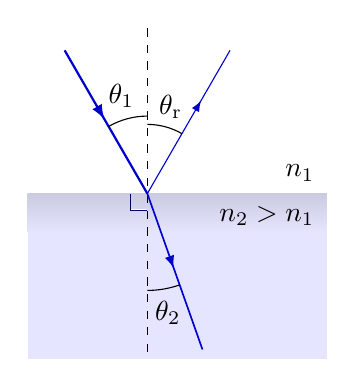
\begin{tikzpicture}
  \def\L{3.8}   % width interface
  \def\l{2.1}   % length ray
  \def\t{0.5}   % depth glass gradient
  \def\h{2.1}   % bisector height
  \def\f{0.4}   % fraction of interface to the left
  \def\na{1.0}  % air
  \def\ng{1.5}  % glass
  \def\anga{30} % angle of incident ray
  \def\angg{asin(\na/\ng*sin(\anga))}
  \coordinate (O) at (0,0);            % point of contact
  \coordinate (I) at (90+\anga:\l);    % point incident (top left)
  \coordinate (M) at (90-\anga:\l);    % point reflected (top right)
  \coordinate (F) at ({-90+\angg}:\l); % point refracted (bottom)
  \coordinate (L) at (-\f*\L,0);       % left point interface
  \coordinate (R) at ({(1-\f)*\L},0);  % right point interface
  \coordinate (T) at (0,\h);           % top middle point (bisector)
  \coordinate (B) at (0,-1.0*\h);      % bottom middle point (bisector)
  
  % MEDIUM
  \fill[glass] (L) rectangle++ (\L,-\t); % glass gradient
  \fill[glasscol] (-\f*\L,-0.99*\t) rectangle ({1-\f)*\L},-\h); % glass bulk
  %\fill[glass] (L) rectangle (\L/2,-\h);
  \node[above left=1] at (R) {$n_1$};
  \node[below left=1] at (R) {$n_2>n_1$};
  
  % LINES
  \draw[dashed] (T) -- (B); % bisector
  \draw[light beam={0.48}] (I) -- (O); % incoming ray
  \draw[light beam={0.65},line width=0.4] (O) -- (M); % reflected ray
  \draw[light beam={0.48},line width=0.6] (O) -- (F); % refracted ray
  
  % ANGLES
  \draw pic["$\theta_1$",draw=black,angle radius=28,angle eccentricity=1.3] {angle = T--O--I}; %\contour{white}{
  \draw pic["$\theta_\mathrm{r}$",draw=black,angle radius=25,angle eccentricity=1.3] {angle = M--O--T};
  \draw pic["$\theta_2$",draw=black,angle radius=35,angle eccentricity=1.25] {angle = B--O--F};
  \rightAngle{B}{O}{L}{0.3}
  
\end{tikzpicture}


% REFRACTION: Hughens' principle
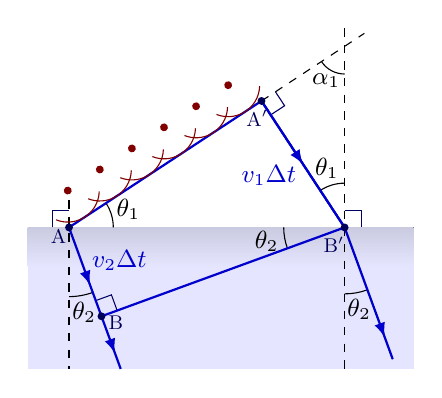
\begin{tikzpicture}
  \small
  \def\N{6}    % number of wavefronts
  \def\r{0.4}  % wavefront radius
  \def\w{3.5}  % width
  \def\h{2.3}  % height
  \def\d{1.8}  % depth
  \def\t{0.5}  % thickness
  \def\l{1.78} % length light beam
  \def\p{0.05} % point size
  \def\ang{atan(\h/\w)}
  \def\ymin{-0.15*\w}
  \def\ymax{ 1.25*\w}
  \def\na{1.0} % air
  \def\ng{1.6} % glass
  \def\anga{20}
  \def\angg{asin(\na/\ng*\h/sqrt(\h^2+\w^2))}
  \def\sangg{\na/\ng*\h/sqrt(\h^2+\w^2)}
  \coordinate (O) at (0,0);
  \coordinate (WR) at (\w,0);
  \coordinate (WT) at (\w,\h);
  \coordinate (L) at (\ymin,0);
  \coordinate (R) at (\ymax,0);
  \coordinate (T) at (\w, 1.10*\h);
  \coordinate (B) at (\w,-\d);
  \coordinate (BL) at (0,-\d);
  \coordinate (TL) at (0,0.15*\h);
  \coordinate (P) at ($(WT)!(WR)!(O)$);
  \coordinate (F) at ({\w+\l*cos(-90+\angg)},{\l*sin(-90+\angg)});
  \coordinate (VT) at ({\w*\sangg*\sangg},{-\w*\sangg*cos(\angg)});
  %\coordinate (VI) at ({\w+\l*cos(180+\angg)},{\l*sin(180+\angg)});
  
  % MEDIUM
  \fill[glass] (L) rectangle (\ymax,-\t);
  \fill[glasscol] (\ymin,-0.99*\t) rectangle (\ymax,-\d);
  
  % ANGLE
  \rightAngle{WT}{WR}{R}{0.3}
  \rightAngle{WT}{P}{WR}{0.3}
  \rightAngle{O}{VT}{WR}{0.3}
  \rightAngle{L}{O}{TL}{0.3}
  \draw pic["$\theta_1$",draw=black,angle radius=16,angle eccentricity=1.4] {angle = R--O--WT};
  \draw pic["$\theta_1$",draw=black,angle radius=16,angle eccentricity=1.4] {angle = WT--WR--P};
  \draw pic["$\theta_2$",draw=black,angle radius=24,angle eccentricity=1.25] {angle = B--WR--F};
  \draw pic["$\alpha_1$",draw=black,angle radius=10,angle eccentricity=1.4] {angle = O--WT--WR};
  \draw pic["$\theta_2$",draw=black,angle radius=22,angle eccentricity=1.3] {angle = L--WR--VT};
  \draw pic["$\theta_2$",draw=black,angle radius=25,angle eccentricity=1.25] {angle = BL--O--VT};
  
  % LINES
  \draw[dashed] (TL) -- (BL);
  \draw[dashed] (T) -- (B);
  \draw[dashed] (P) -- (WT) --++ ({\ang}:0.3);
  \draw[light beam={0.65}] (O) -- (VT) node[midway,above=4,right=-1] {$v_2 \Delta t$};
  \draw[light beam={0.70}] (VT) --++ ({\angg-90}:0.4*\l);
  \draw[] (P) -- (WR) -- (F);
  \draw[light beam={0.50}] (P) -- (WR) node[midway,above=2,below left=-1] {$v_1 \Delta t$};
  \draw[light beam={0.92}] (P) -- (WR) -- (F);
  %\draw[] (WT) -- (WR);
  \draw[myblue,thick] (O) -- (P);
  \draw[myblue,thick] (VT) -- (WR);
  
  \fill[mydarkblue] (O) circle (\p) node[scale=0.8,below left=-2] {A};
  \fill[mydarkblue] (P) circle (\p) node[scale=0.8,left=2,below=1] {A$'$};
  \fill[mydarkblue] (VT) circle (\p) node[scale=0.8,below=3,right=0] {B};
  \fill[mydarkblue] (WR) circle (\p) node[scale=0.8,right=4,below left=1] {B$'$};
  
  % WAVE FRONTS
%  \foreach \i [evaluate={\x=-\r*sin(\ang)+\i*\w/(\N+1);
%                         \y=\r*cos(\ang)+\i*\h/(\N+1);}] in {1,...,\N}{
%    \pic[myred,rotate=\ang-90] at (\x,\y) {wavefront={ang={55}}};
%  }
  \foreach \i [evaluate={\f=(\i-0.5)/\N;}] in {1,...,\N}{
    \pic[myred,rotate=\ang-90] at ($(O)!\f!(P)+({\ang+90}:\r)$) {wavefront={ang={55}}};
  }
  
\end{tikzpicture}


% INTERNAL REFLECTION: almost
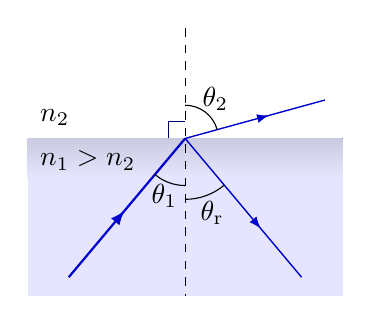
\begin{tikzpicture}
  \def\L{4.0}
  \def\l{2.3}
  \def\t{0.5}
  \def\h{2.0}
  \def\f{0.5}
  \def\na{1.0} % air
  \def\ng{1.5} % glass
  \def\angg{40} % asin(1/1.5)*180/pi
  \def\anga{asin(\ng/\na*sin(\angg))}
  \coordinate (O) at (0,0);
  \coordinate (I) at (-90-\angg:\l);
  \coordinate (M) at (-90+\angg:\l);
  \coordinate (F) at ({90-\anga}:0.8*\l);
  \coordinate (L) at (-\f*\L,0);
  \coordinate (R) at ({(1-\f)*\L},0);
  \coordinate (T) at (0,0.7*\h);
  \coordinate (B) at (0,-\h);
  
  % MEDIUM
  \fill[glass] (L) rectangle++ (\L,-\t); % glass gradient
  \fill[glasscol] (-\f*\L,-0.99*\t) rectangle ({1-\f)*\L},-\h);
  %\fill[glass] (L) rectangle (\L/2,-\h);
  \node[above right=1] at (L) {$n_2$};
  \node[below right=1] at (L) {$n_1>n_2$};
  
  % LINES
  \draw[dashed] (T) -- (B);
  \draw[light beam={0.48}] (I) -- (O);
  \draw[light beam={0.65},line width=0.5] (O) -- (M);
  \draw[light beam={0.60},line width=0.5] (O) -- (F);
  
  % ANGLES
  \draw pic["$\theta_1$",draw=black,angle radius=17,angle eccentricity=1.3] {angle = I--O--B}; %\contour{white}{
  \draw pic["$\theta_\mathrm{r}$",draw=black,angle radius=22,angle eccentricity=1.3] {angle = B--O--M};
  \draw pic["$\theta_2$",draw=black,angle radius=12,angle eccentricity=1.5] {angle = F--O--T};
  \rightAngle{L}{O}{T}{0.3}
  
\end{tikzpicture}


% INTERNAL REFLECTION: critical
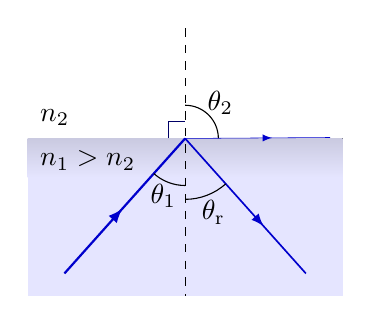
\begin{tikzpicture}
  \def\L{4.0}
  \def\l{2.3}
  \def\t{0.5}
  \def\h{2.0}
  \def\f{0.5}
  \def\na{1.0} % air
  \def\ng{1.5} % glass
  \def\angg{41.804} % asin(1/1.5)*180/pi
  \def\anga{asin(\ng/\na*sin(\angg))}
  \coordinate (O) at (0,0);
  \coordinate (I) at (-90-\angg:\l);
  \coordinate (M) at (-90+\angg:\l);
  \coordinate (F) at ({90-\anga}:0.8*\l);
  \coordinate (L) at (-\f*\L,0);
  \coordinate (R) at ({(1-\f)*\L},0);
  \coordinate (T) at (0,0.7*\h);
  \coordinate (B) at (0,-\h);
  
  % MEDIUM
  \fill[glass] (L) rectangle++ (\L,-\t);
  \fill[glasscol] (-\f*\L,-0.99*\t) rectangle ({1-\f)*\L},-\h);
  %\fill[glass] (L) rectangle (\L/2,-\h);
  \node[above right=1] at (L) {$n_2$};
  \node[below right=1] at (L) {$n_1>n_2$};
  
  % LINES
  \draw[dashed] (T) -- (B);
  \draw[light beam={0.48}] (I) -- (O);
  \draw[light beam={0.65},line width=0.6] (O) -- (M);
  \draw[light beam={0.60},line width=0.2] (O) -- (F);
  
  % ANGLES
  \draw pic["$\theta_1$",draw=black,angle radius=17,angle eccentricity=1.3] {angle = I--O--B}; %\contour{white}{
  \draw pic["$\theta_\mathrm{r}$",draw=black,angle radius=22,angle eccentricity=1.3] {angle = B--O--M};
  \draw pic["$\theta_2$",draw=black,angle radius=12,angle eccentricity=1.5] {angle = F--O--T};
  \rightAngle{L}{O}{T}{0.3}
  
\end{tikzpicture}


% BREWSTER/POLARIZATION ANGLE
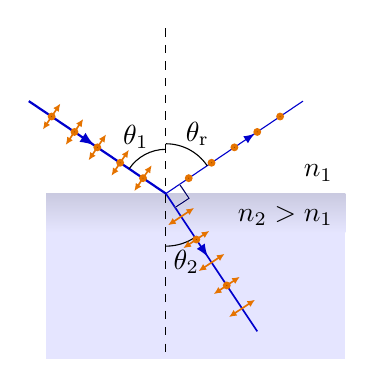
\begin{tikzpicture}
  \def\A{0.2}
  \def\L{3.8}
  \def\l{2.1}
  \def\t{0.5}
  \def\h{2.1}
  \def\f{0.4}
  \def\na{1.0} % air
  \def\ng{1.5} % glass
  \def\anga{56} % atan(1.5)*180/pi
  \def\angg{asin(\na/\ng*sin(\anga))}
  \def\N{5}
  \coordinate (O) at (0,0);
  \coordinate (I) at (90+\anga:\l);
  \coordinate (M) at (90-\anga:\l);
  \coordinate (F) at ({-90+\angg}:\l);
  \coordinate (L) at (-\f*\L,0);
  \coordinate (R) at ({(1-\f)*\L},0);
  \coordinate (T) at (0,\h);
  \coordinate (B) at (0,-1.0*\h);
  \def\dot#1{
    \fill[Ecol] (#1) circle (0.05);
    \fill[Ecol!60!black] (#1) circle (0.007);
    %\draw[Ecol!70!black,line width=0.05] (90+\anga:\t) circle (0.03);
  }
  
  % MEDIUM
  \fill[glass] (L) rectangle++ (\L,-\t);
  \fill[glasscol] (-\f*\L,-0.99*\t) rectangle ({1-\f)*\L},-\h);
  %\fill[glass] (L) rectangle (\L/2,-\h);
  \node[above left=1] at (R) {$n_1$};
  \node[below left=1] at (R) {$n_2>n_1$};
  
  % LINES
  \draw[dashed] (T) -- (B);
  \draw[light beam={0.48}] (I) -- (O);
  \draw[light beam={0.65},line width=0.4] (O) -- (M);
  \draw[light beam={0.46},line width=0.6] (O) -- (F);
  
  % ANGLES
  \draw pic["$\theta_1$",draw=black,angle radius=16,angle eccentricity=1.45] {angle = T--O--I}; %\contour{white}{
  \draw pic["$\theta_\mathrm{r}$",draw=black,angle radius=18,angle eccentricity=1.35] {angle = M--O--T};
  \draw pic["$\theta_2$",draw=black,angle radius=19,angle eccentricity=1.35] {angle = B--O--F};
  \rightAngle{M}{O}{F}{0.3}
  
  % VECTORS
  \foreach \i [evaluate={\t=\i*\l/(\N+1);}] in {1,...,\N}{
    \draw[Evec] (90+\anga:\t)++(\anga+180:\A) --++ (\anga:2*\A); % incident
    \dot{90+\anga:\t} % incident
    %\draw[Evec] (90-\anga:\t)++(180-\anga:\A) --++ (-\anga:2*\A); % reflected
    %\dot{{-90+\angg}:\t} % refracted
    \draw[Evec] ({-90+\angg}:\t)++({-180+\angg}:\A) --++ ({\angg}:2*\A); % reflected
    \dot{{90-\anga}:\t} % refracted
  }
  \dot{{-90+\angg}:{\l*2/(\N+1)}} % refracted
  \dot{{-90+\angg}:{\l*4/(\N+1)}} % refracted
  
\end{tikzpicture}


% REFLECTION & REFRACTION - Brewster angle
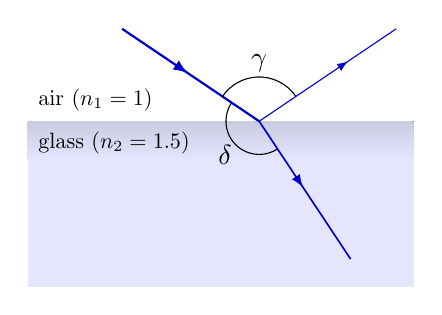
\begin{tikzpicture}
  \def\L{4.9}   % width interface
  \def\l{2.1}   % length ray
  \def\t{0.5}   % depth glass gradient
  \def\h{2.1}   % bisector height
  \def\f{0.6}   % fraction of interface to the left
  \def\na{1.0}  % air
  \def\ng{1.5}  % glass
  \def\anga{56} % angle of incident ray
  \def\angg{asin(\na/\ng*sin(\anga))}
  \coordinate (O) at (0,0);            % point of contact
  \coordinate (I) at (90+\anga:\l);    % point incident (top left)
  \coordinate (M) at (90-\anga:\l);    % point reflected (top right)
  \coordinate (F) at ({-90+\angg}:\l); % point refracted (bottom)
  \coordinate (L) at (-\f*\L,0);       % left point interface
  \coordinate (R) at ({(1-\f)*\L},0);  % right point interface
  \coordinate (T) at (0,\h);           % top middle point (bisector)
  \coordinate (B) at (0,-1.0*\h);      % bottom middle point (bisector)
  
  % MEDIUM
  \fill[glass] (L) rectangle++ (\L,-\t); % glass gradient
  \fill[glasscol] (-\f*\L,-0.99*\t) rectangle ({1-\f)*\L},-\h); % glass bulk
  \node[above right=1,scale=0.8] at (L) {air ($n_1=1$)};
  \node[below right=1,scale=0.8] at (L) {glass ($n_2=1.5$)};
  
  % LINES
  %\draw[dashed] (T) -- (B); % bisector
  \draw[light beam={0.48}] (I) -- (O); % incoming ray
  \draw[light beam={0.65},line width=0.4] (O) -- (M); % reflected ray
  \draw[light beam={0.48},line width=0.6] (O) -- (F); % refracted ray
  
  % ANGLES
  \draw pic["$\gamma$",draw=black,angle radius=16,angle eccentricity=1.30] {angle = M--O--I};
  \draw pic["$\delta$",draw=black,angle radius=12,angle eccentricity=1.45] {angle = I--O--F};
  
\end{tikzpicture}



\end{document}